
\newpage
\setlength{\voffset}{-3cm}

\begin{center}
\section{\textbf{\huge{Form}}}

\Large{Use Cases}
\end{center}

%--------START EDITING HERE FOR HANDLING---------
%Maria

%--------Form Use case---------
\subsection{createNewForm}
\textbf{Description:}
This use-case allows for the addition of a new form on to the system by first building the form with a form builder tool.
\subsubsection{Prioritization:}
Important
\subsubsection{Conditions and Data Structures:}
\textbf{Pre-Conditions:}
\begin{itemize}
	\item User has Administrator rights on the system.
	\item Form must not exist on the system.
\end{itemize}

\textbf{Post-Conditions:}	
\begin{itemize}
	\item New form is created and persisted to Database
\end{itemize}
\subsubsection{Service Contract:} 
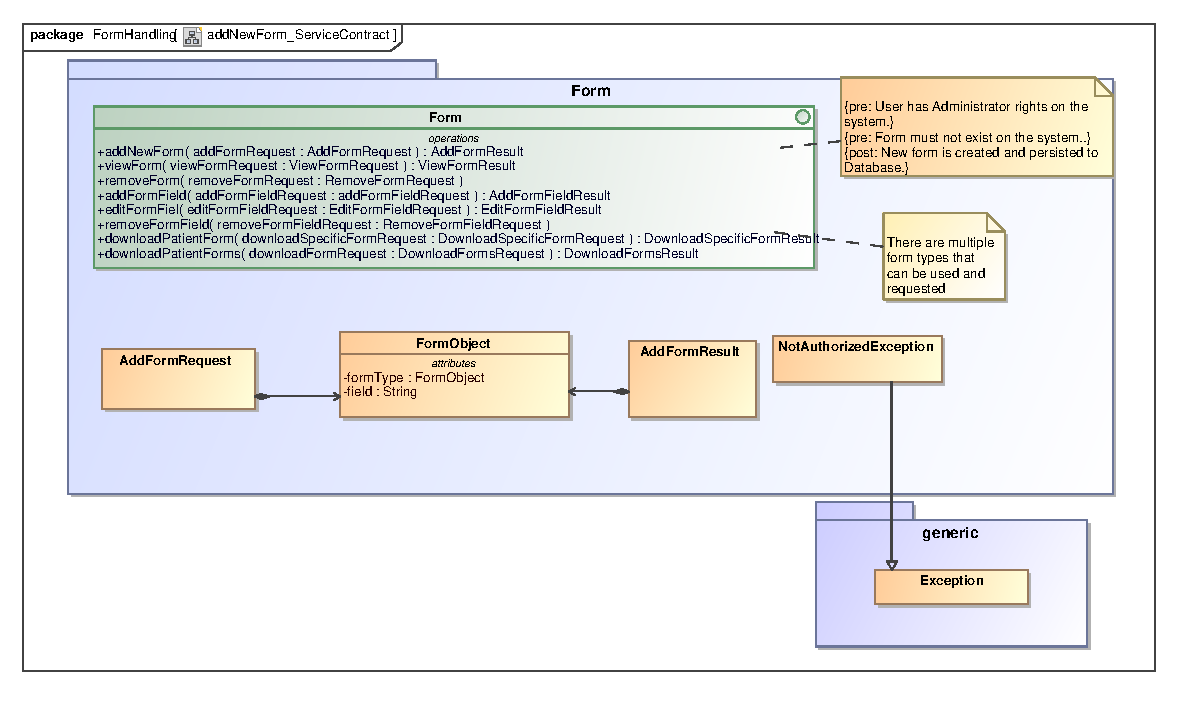
\includegraphics[width=1\linewidth]{./Graphics/FormUseCaseDiagrams/addNewForm_ServiceContract}
%\subsubsection{Required Functionality:}
\subsubsection{Process Specifications:} 
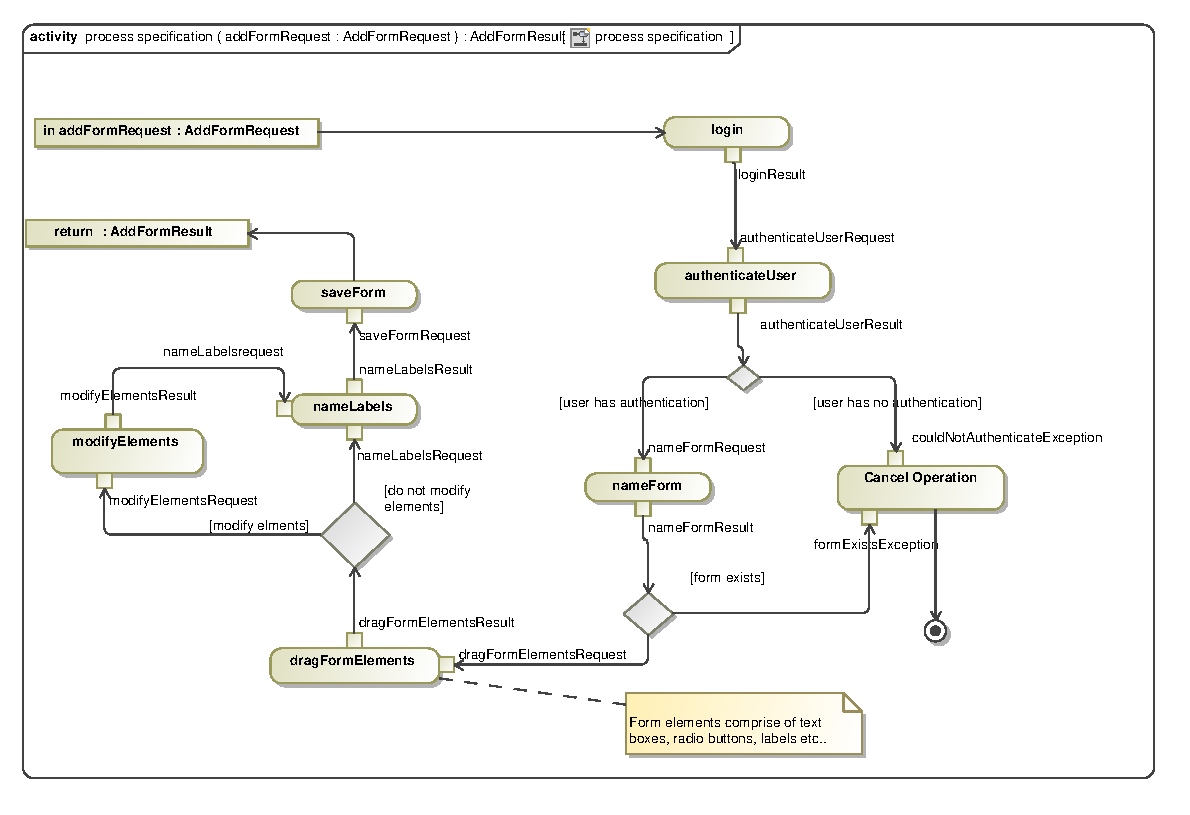
\includegraphics[width=1\linewidth]{./Graphics/FormUseCaseDiagrams/processspecification_AddForm}



\subsection{viewForm}
\textbf{Description:}
This use-case allows for viewing of a form.
\subsubsection{Prioritization:}
Important
\subsubsection{Conditions and Data Structures:}
\textbf{Pre-Conditions:}
\begin{itemize}
	\item Form must exist
\end{itemize}

\textbf{Post-Conditions:}	
\begin{itemize}
	\item Form is displayed on GUI
\end{itemize}
\subsubsection{Service Contract:} 
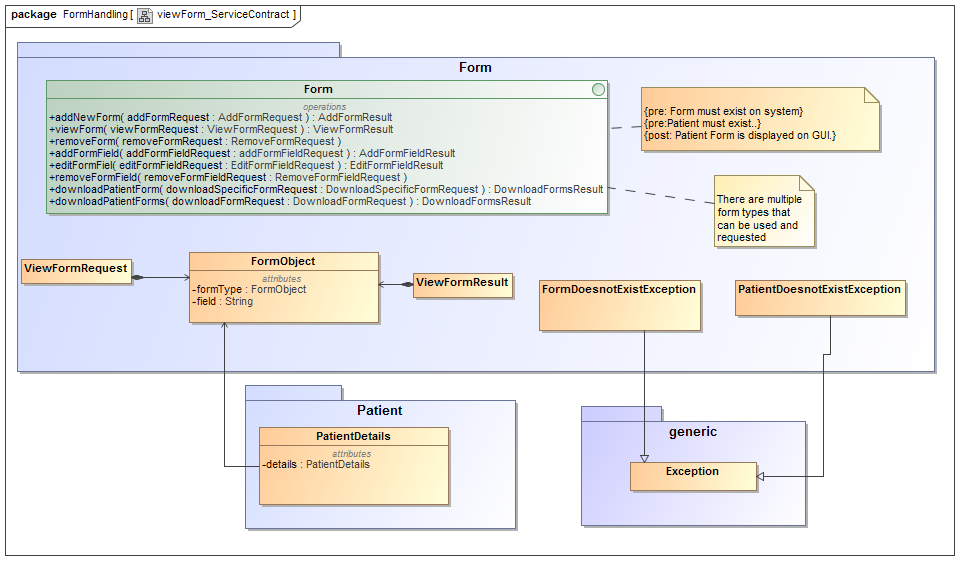
\includegraphics[width=1\linewidth]{./Graphics/FormUseCaseDiagrams/viewForm_ServiceContract}
%\subsubsection{Required Functionality:} 
\subsubsection{Process Specifications:} 
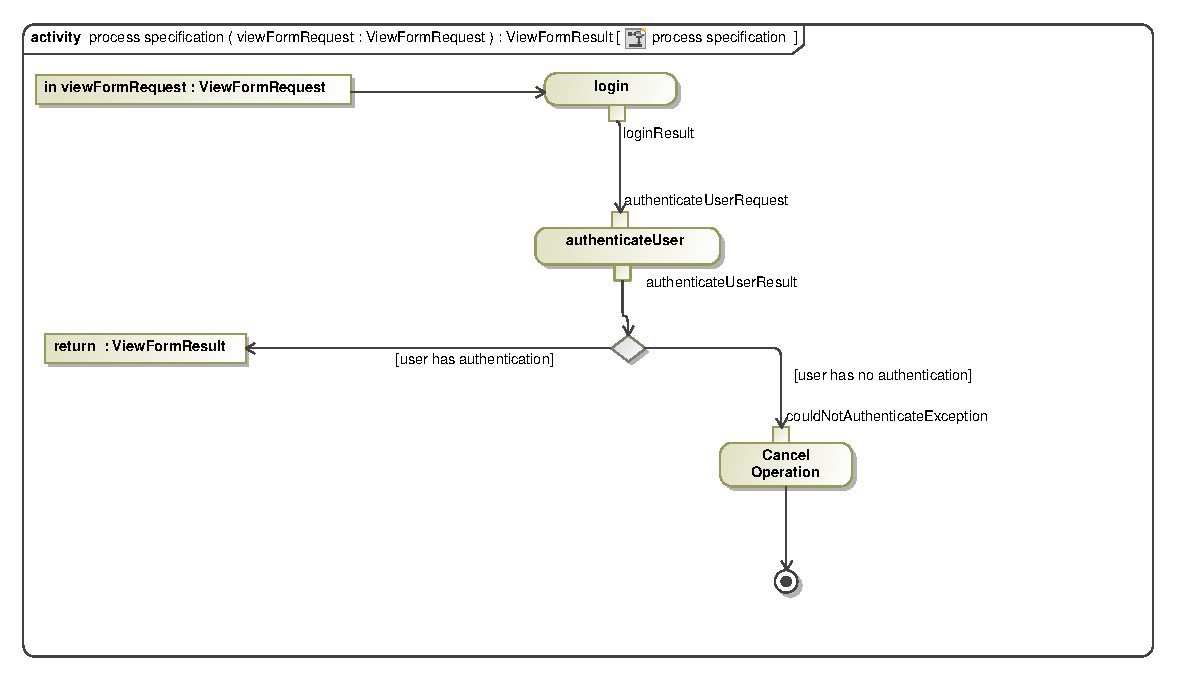
\includegraphics[width=1\linewidth]{./Graphics/FormUseCaseDiagrams/processspecification_ViewForm}

%\textbf{Use case diagram for Login}\\
%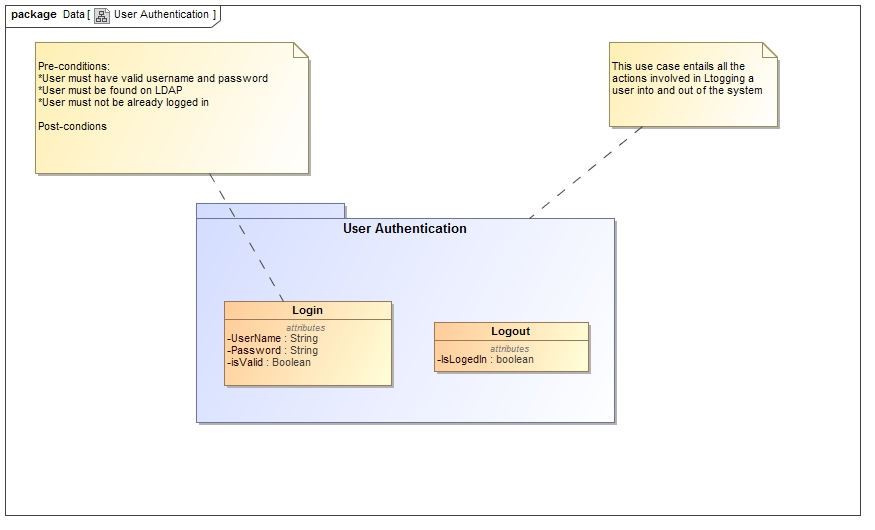
\includegraphics[width=1\linewidth]{./Images/Author/Login.jpg}\\





\subsection{removeForm}
\textbf{Description:}
This use-case allows for the logical removal of a form, in that the form will be archived on the system so that it can be retrieved later if needed.
\subsubsection{Prioritization:}
Important
\subsubsection{Conditions and Data Structures:}
\textbf{Pre-Conditions:}
\begin{itemize}
	\item User has Administrator rights on the system.
	\item Form to be removed must exist.
	\item The editable form fields must not be filled in at time for deletion
\end{itemize}

\textbf{Post-Conditions:}	
\begin{itemize}
	\item Form is archived
\end{itemize}
\subsubsection{Service Contract:} 
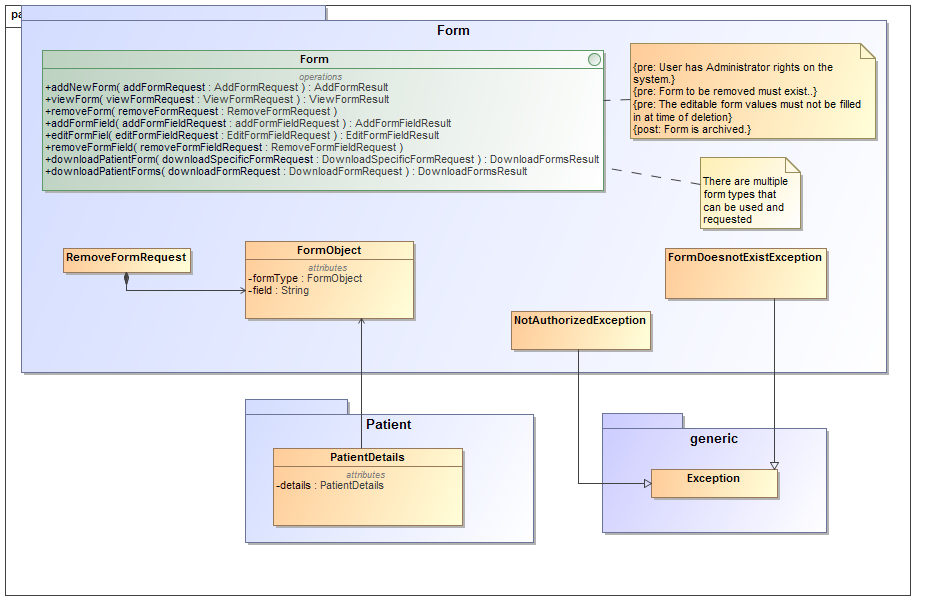
\includegraphics[width=1\linewidth]{./Graphics/FormUseCaseDiagrams/removeForm_ServiceContract}
%\subsubsection{Required Functionality:} 
\subsubsection{Process Specifications:} 
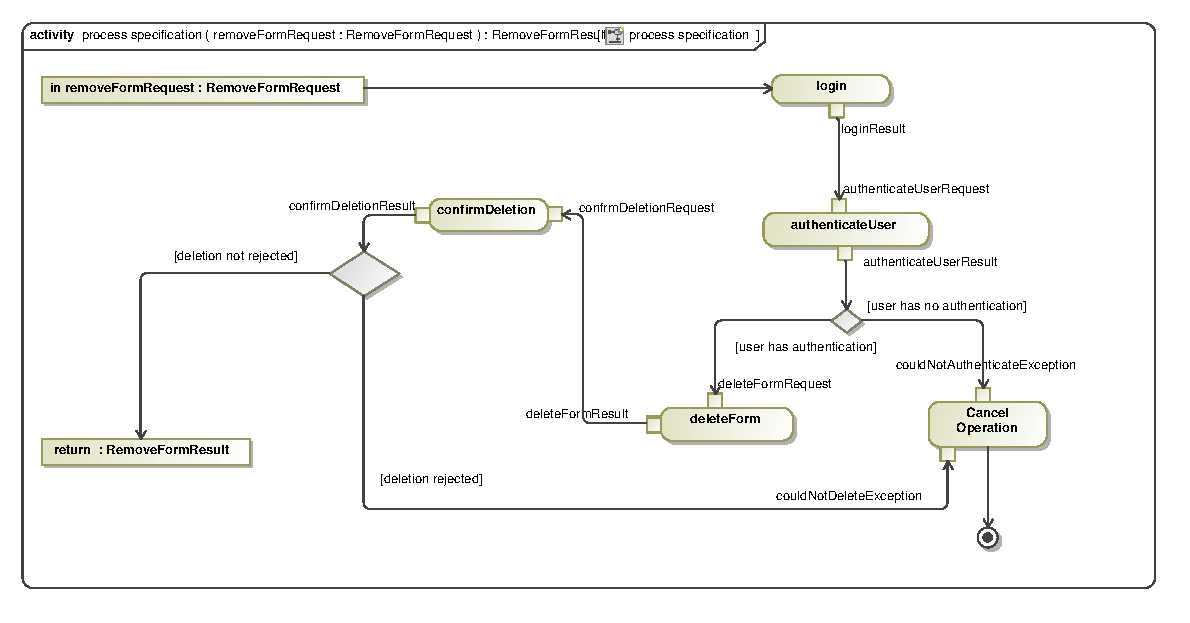
\includegraphics[width=1\linewidth]{./Graphics/FormUseCaseDiagrams/processspecification_RemoveForm}

%\textbf{Use case diagram for Login}\\
%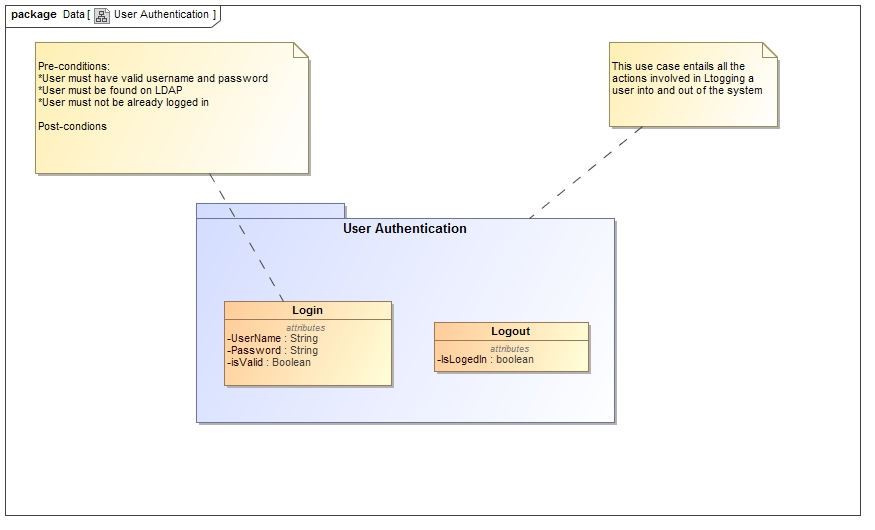
\includegraphics[width=1\linewidth]{./Images/Author/Login.jpg}\\






%\subsection{editForm}
\subsection{addFormField}
\textbf{Description:}
This use-case allows for the addition of a new form field into a currently existing form
\subsubsection{Prioritization:}
Nice-to-Have
\subsubsection{Conditions and Data Structures:}
\textbf{Pre-Conditions:}
\begin{itemize}
	\item User has Administrator rights on the system.
	\item Form to be edited must exist on system.
\end{itemize}

\textbf{Post-Conditions:}	
\begin{itemize}
	\item Field is added to GUI and persisted to DB
\end{itemize}
\subsubsection{Service Contract:} 
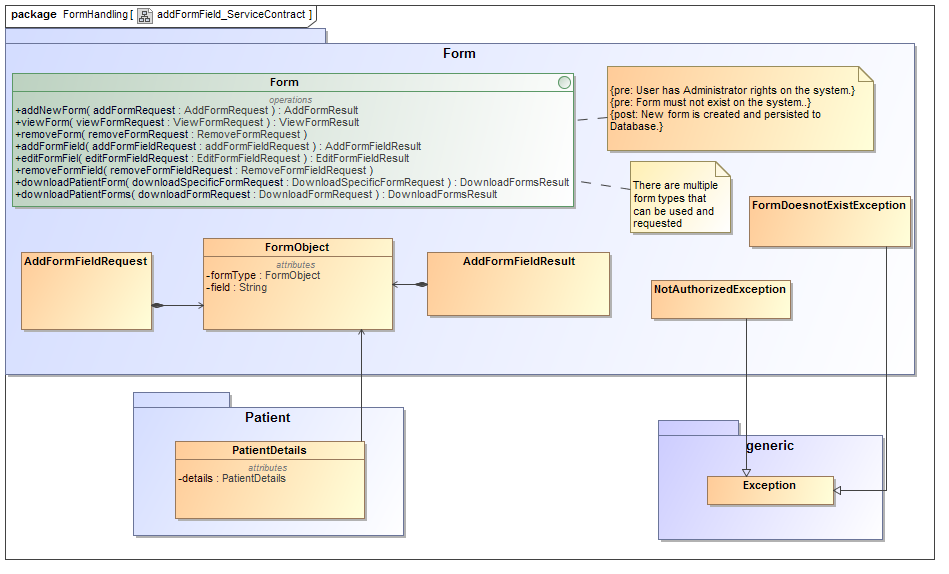
\includegraphics[width=1\linewidth]{./Graphics/FormUseCaseDiagrams/addFormField_ServiceContract}
%\subsubsection{Required Functionality:} 
\subsubsection{Process Specifications:} 
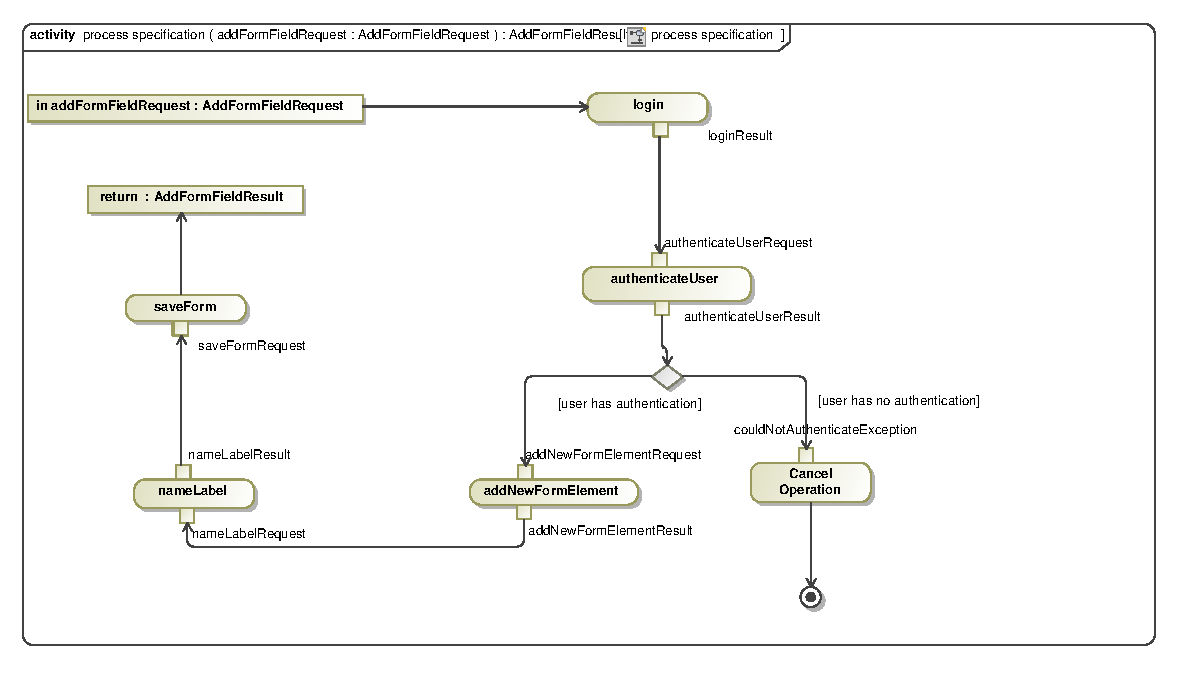
\includegraphics[width=1\linewidth]{./Graphics/FormUseCaseDiagrams/processspecification_AddFormField}

%\textbf{Use case diagram for Login}\\
%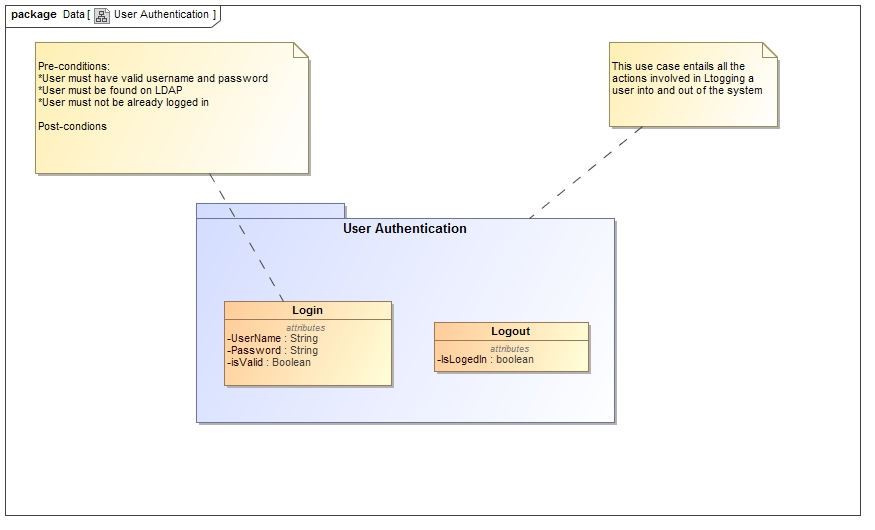
\includegraphics[width=1\linewidth]{./Images/Author/Login.jpg}\\





\subsection{editFormField}
\textbf{Description:}
This use-case allows for the editing of the field of a specific form that is on the system.
\subsubsection{Prioritization:}
Nice-to-Have
\subsubsection{Conditions and Data Structures:}
\textbf{Pre-Conditions:}
\begin{itemize}
	\item User has Administrator rights on the system.
	\item Field must exist on form.
	\item Form to be edited must exist on system.
\end{itemize}

\textbf{Post-Conditions:}	
\begin{itemize}
	\item Edited field is updated on Form GUI and updated in Database
\end{itemize}
\subsubsection{Service Contract:} 
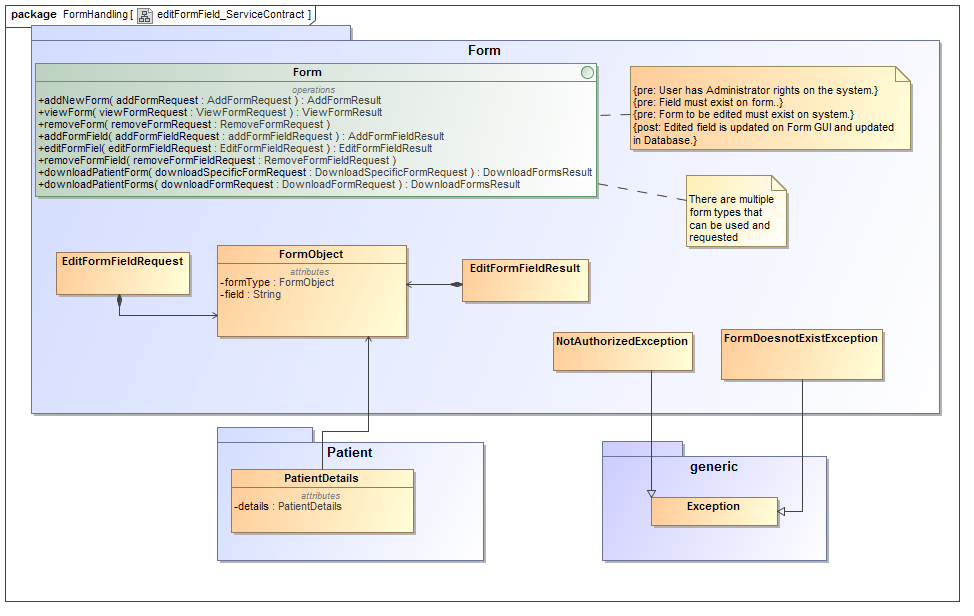
\includegraphics[width=1\linewidth]{./Graphics/FormUseCaseDiagrams/editFormField_ServiceContract}
%\subsubsection{Required Functionality:} 
\subsubsection{Process Specifications:} 
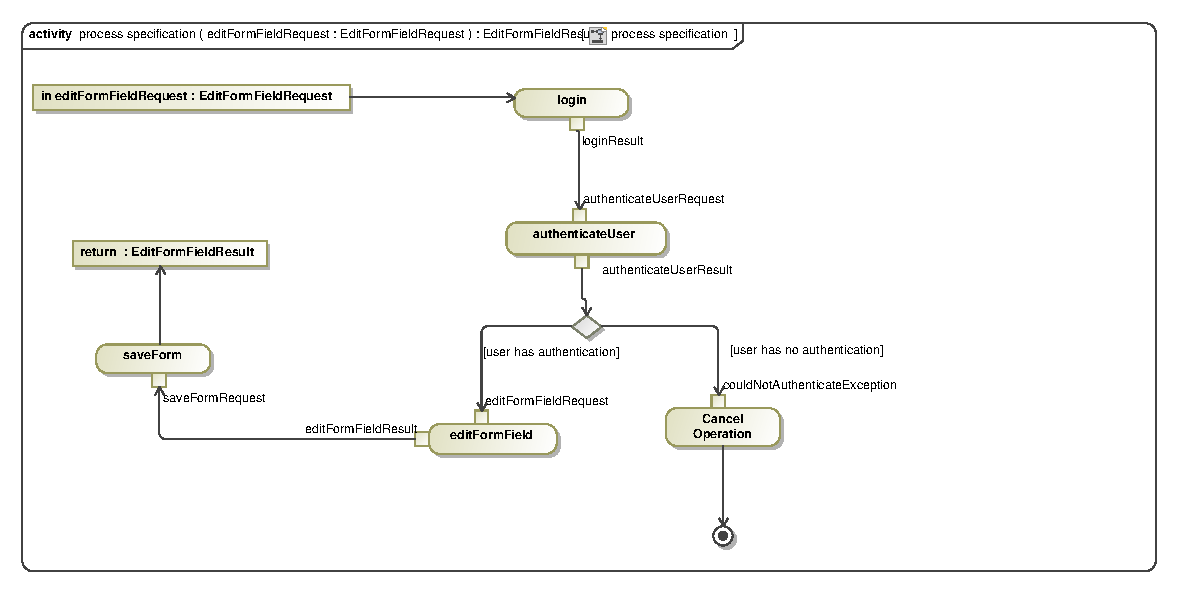
\includegraphics[width=1\linewidth]{./Graphics/FormUseCaseDiagrams/processspecification_editField}

%\textbf{Use case diagram for Login}\\
%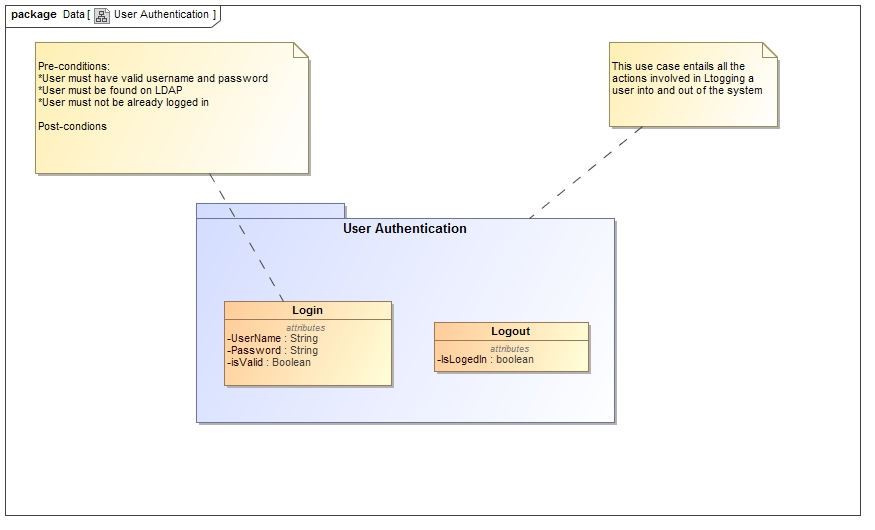
\includegraphics[width=1\linewidth]{./Images/Author/Login.jpg}\\




\subsection{removeFormField}
\textbf{Description:}
This use-case allows for the logical deletion of a form field in that the field will no longer be shown on the GUI but would still be present in the Database.
\subsubsection{Prioritization:}
Nice-to-Have
\subsubsection{Conditions and Data Structures:}
\textbf{Pre-Conditions:}
\begin{itemize}
	\item User has Administrator rights on the system.
	\item Field must exist on form.
	\item Form to be removed must exist on system.
\end{itemize}

\textbf{Post-Conditions:}	
\begin{itemize}
	\item Field is removed from GUI and archived.  
\end{itemize}
\subsubsection{Service Contract:} 
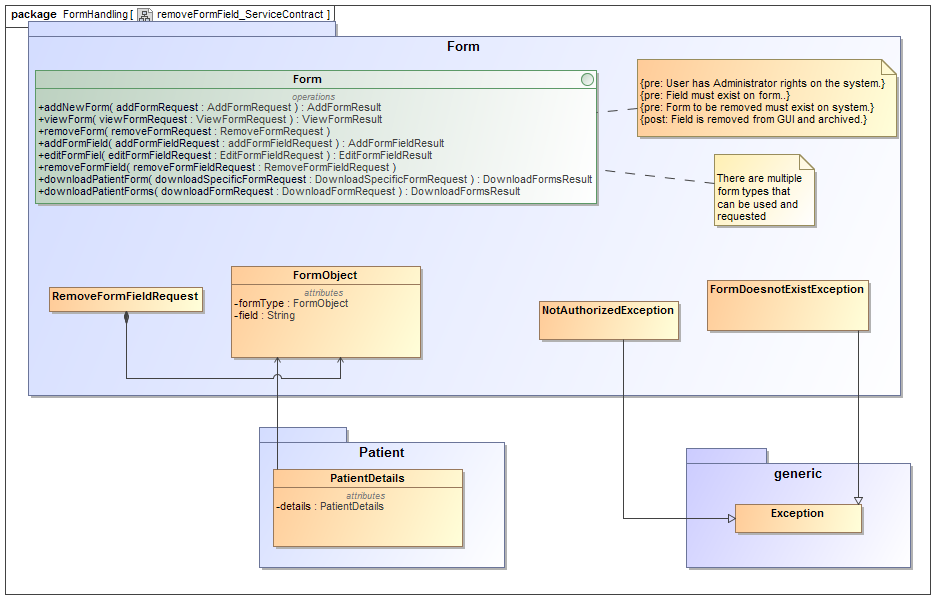
\includegraphics[width=1\linewidth]{./Graphics/FormUseCaseDiagrams/removeFormField_ServiceContract}
%\subsubsection{Required Functionality:} 
\subsubsection{Process Specifications:} 
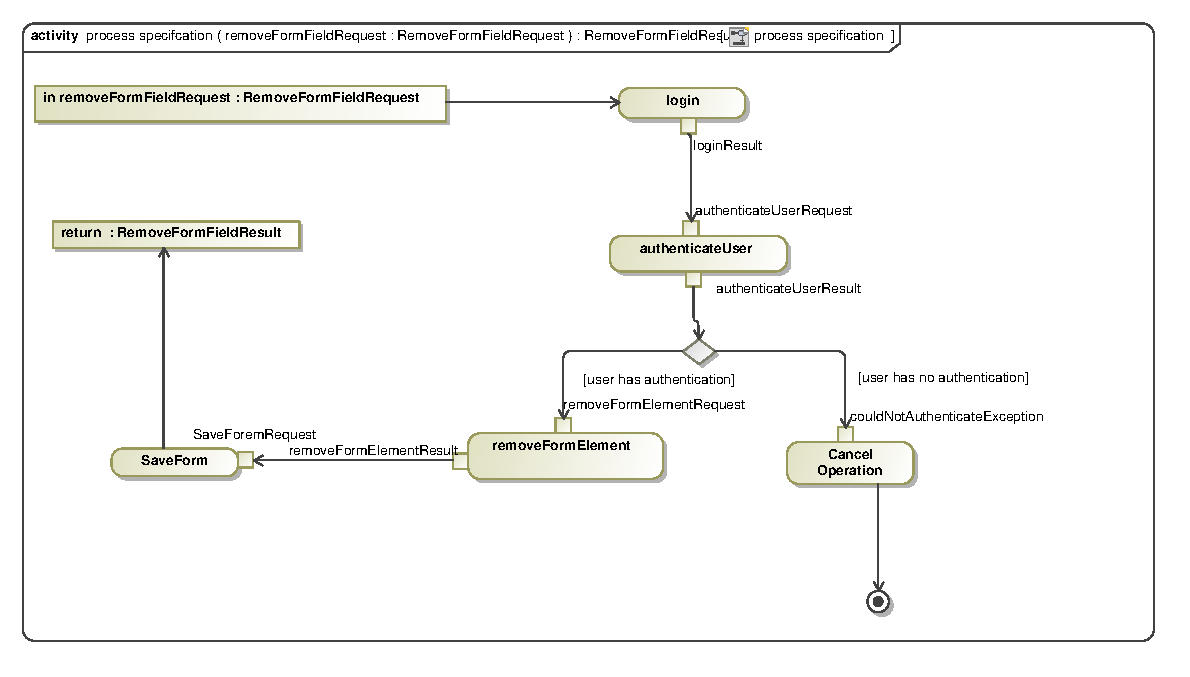
\includegraphics[width=1\linewidth]{./Graphics/FormUseCaseDiagrams/processspecification_RemoveFormField}

%\textbf{Use case diagram for Login}\\
%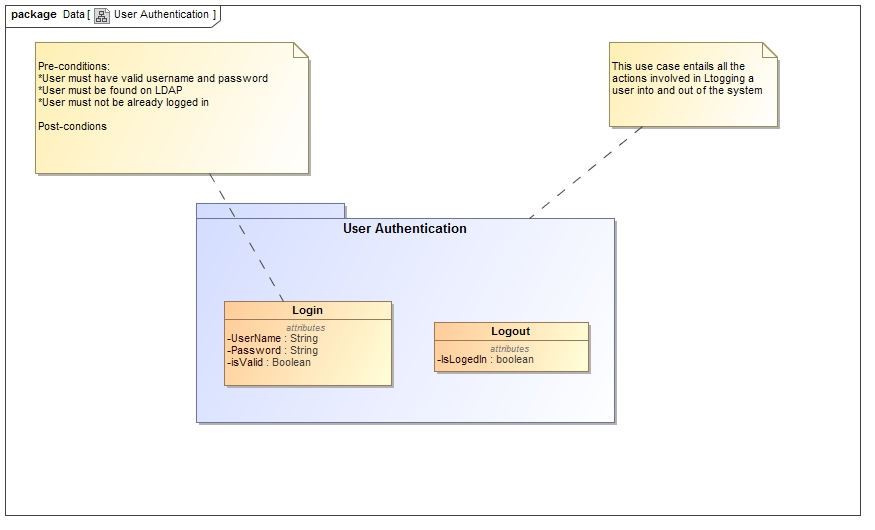
\includegraphics[width=1\linewidth]{./Images/Author/Login.jpg}\\



\subsection{downloadPatientForm} %for a specific form
\textbf{Description:}
This use-case allows for downloading of a particular form associated with the specified patient.
\subsubsection{Prioritization:}
Nice-to-Have
\subsubsection{Conditions and Data Structures:}
\textbf{Pre-Conditions:}
\begin{itemize}
	\item User has Administrator rights on the system.
	\item Form must exist on the system.
	\item Patient must exist on Hospital LDAP.
\end{itemize}

\textbf{Post-Conditions:}	
\begin{itemize}
	\item Form is downloaded from server to local hard drive of user
\end{itemize}
\subsubsection{Service Contract:} 
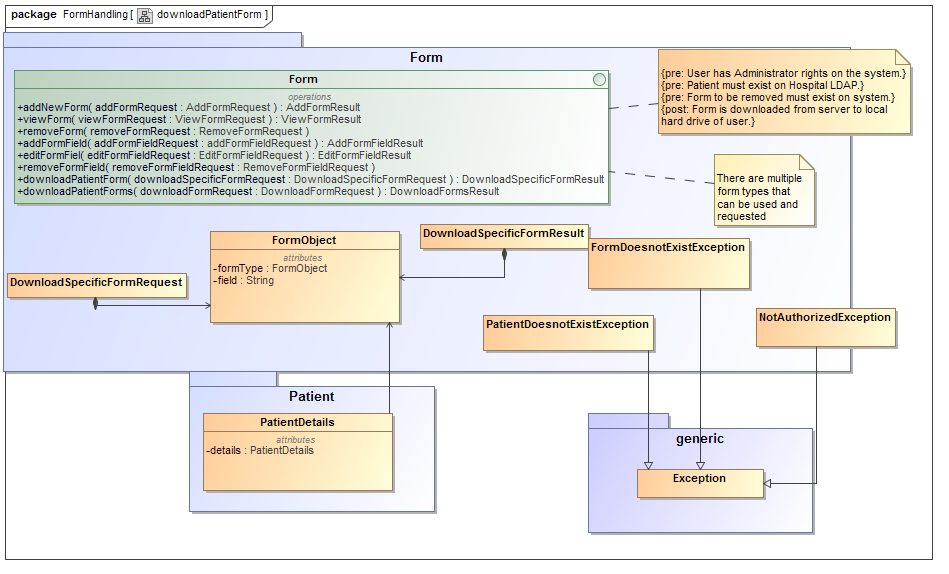
\includegraphics[width=1\linewidth]{./Graphics/FormUseCaseDiagrams/downloadPatientForm}
%\subsubsection{Required Functionality:} 
\subsubsection{Process Specifications:}
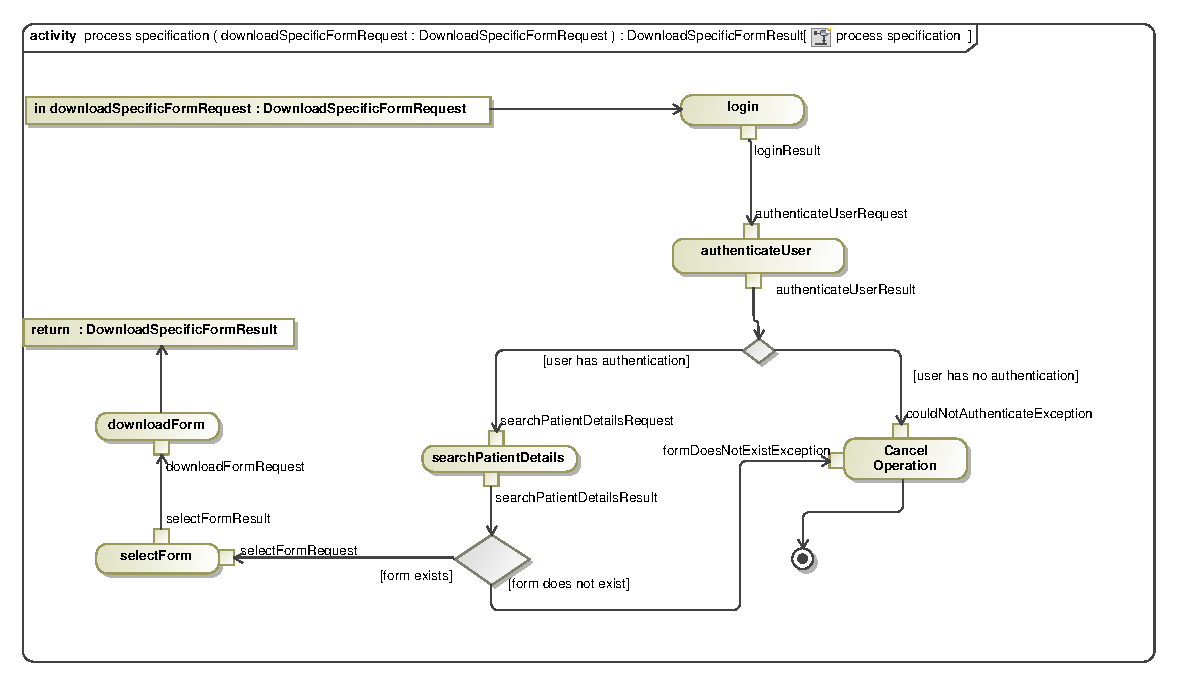
\includegraphics[width=1\linewidth]{./Graphics/FormUseCaseDiagrams/processspecification_DownloadSpecificForm}

%\textbf{Use case diagram for Login}\\
%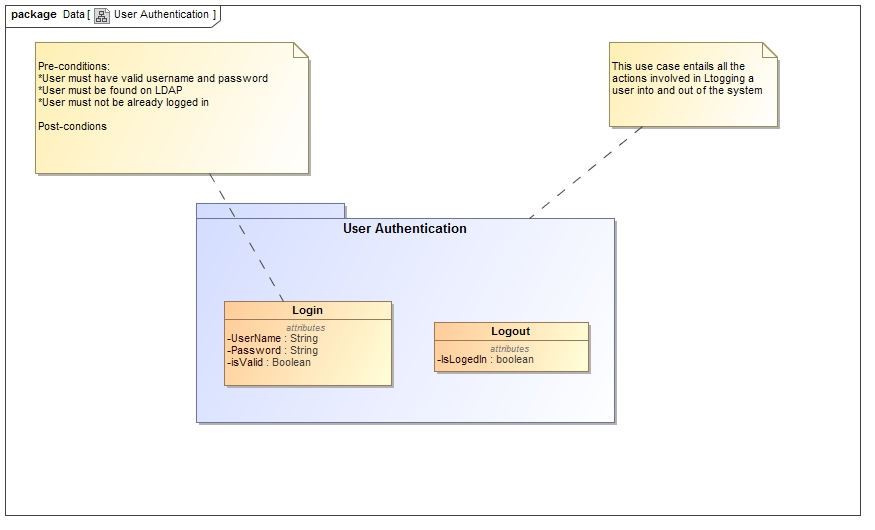
\includegraphics[width=1\linewidth]{./Images/Author/Login.jpg}\\




\subsection{downloadPatientForms} %download all forms
\textbf{Description:}
This use-case allows for downloading of all forms associated with the specified patient.
\subsubsection{Prioritization:}
Nice-to-Have
\subsubsection{Conditions and Data Structures:}
\textbf{Pre-Conditions:}
\begin{itemize}
	\item User has Administrator rights on the system.
	\item Form must exist on the system.
	\item Patient must exist on Hospital LDAP.
	\item Patient information must exist.
\end{itemize}

\textbf{Post-Conditions:}	
\begin{itemize}
	\item Forms are zipped and downloaded from server to local hard drive of user
\end{itemize}
\subsubsection{Service Contract:} 
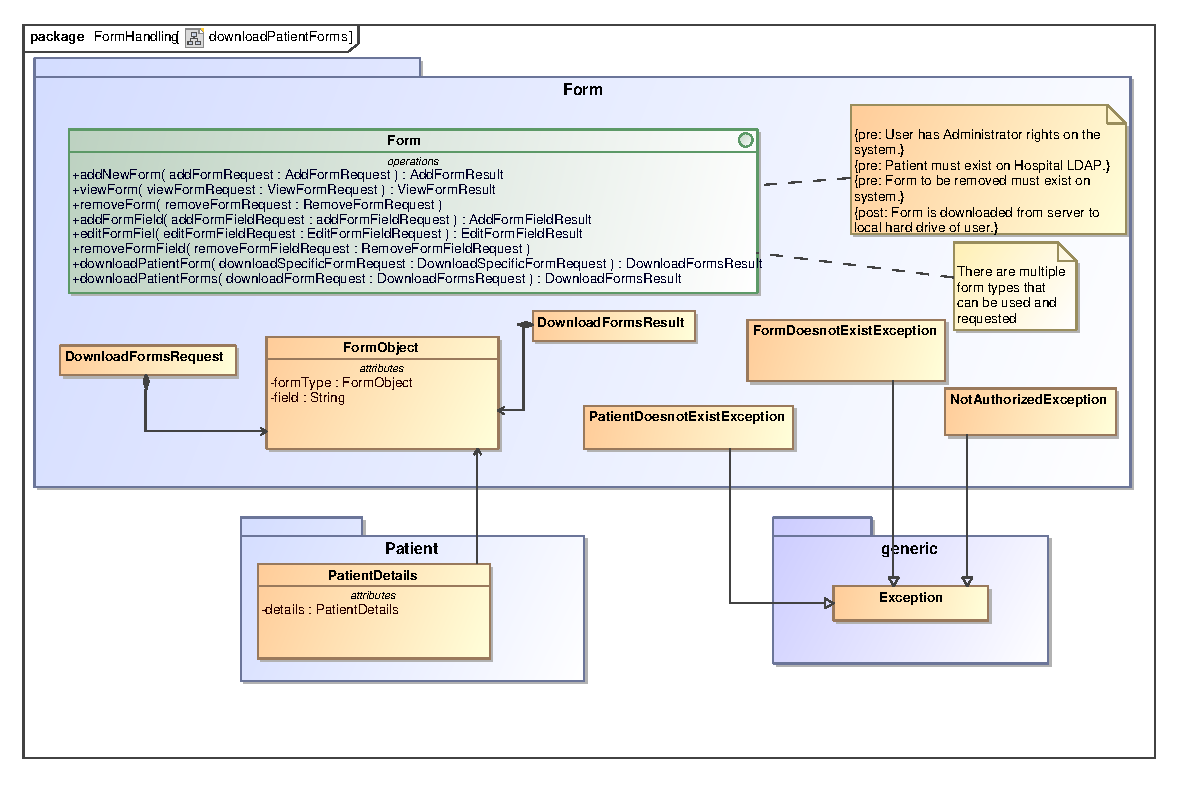
\includegraphics[width=1\linewidth]{./Graphics/FormUseCaseDiagrams/downloadPatientForms}
%\subsubsection{Required Functionality:} 
\subsubsection{Process Specifications:} 
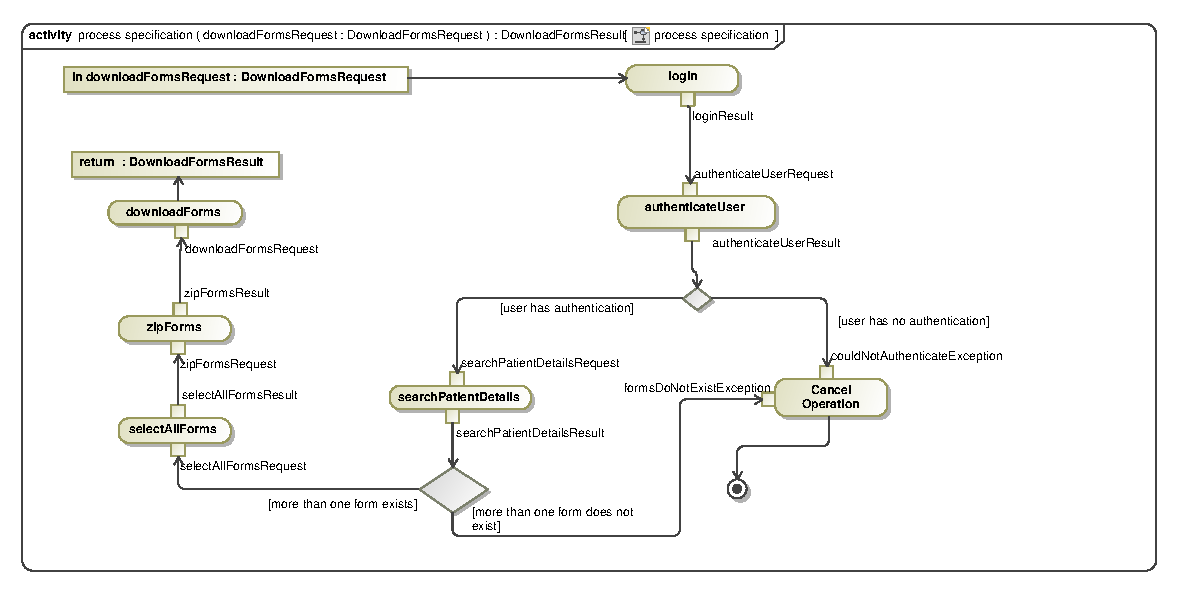
\includegraphics[width=1\linewidth]{./Graphics/FormUseCaseDiagrams/processspecification_DownloadForms}

%\textbf{Use case diagram for Login}\\
%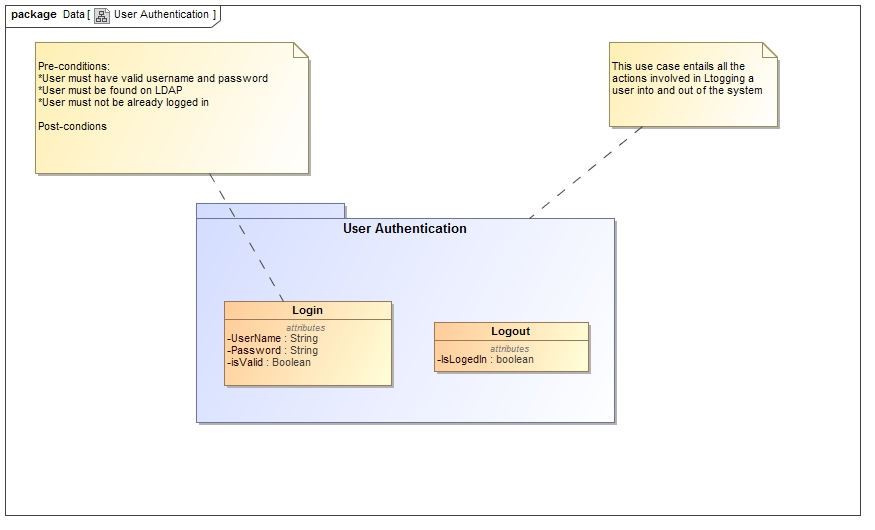
\includegraphics[width=1\linewidth]{./Images/Author/Login.jpg}\\




